\chapter{Hybrid Metaheuristic Approach}

A large number of researchers have recognized the advantages and huge potential of building hybrid metaheuristics. The main motivation for creating hybrid metaheuristics is to exploit the complementary character of different optimization strategies. In fact, choosing an adequate combination of algorithms can be the key to achieving top performance in solving many hard optimization problems \cite{Puchinger2005} \cite{Blum2012}.

The proposed solution makes it possible to create a model that evolves during the test. The proposed solution model uses genetic algorithms, tabu search, and simulated annealing in two different approaches. The study initially investigated the use of these three algorithms. Subsequently, the study will focus in others Population-based and single point search metaheuristics. The first approach uses the three algorithms independently, and the second approach uses the three algorithms collaboratively (hybrid metaheuristic approach).

In the first approach , the algorithms do not share their best individuals among themselves. Each algorithm evolves in a separate way (Fig. \ref{fig:firstaproach}).


\begin{figure}[h]
\centering
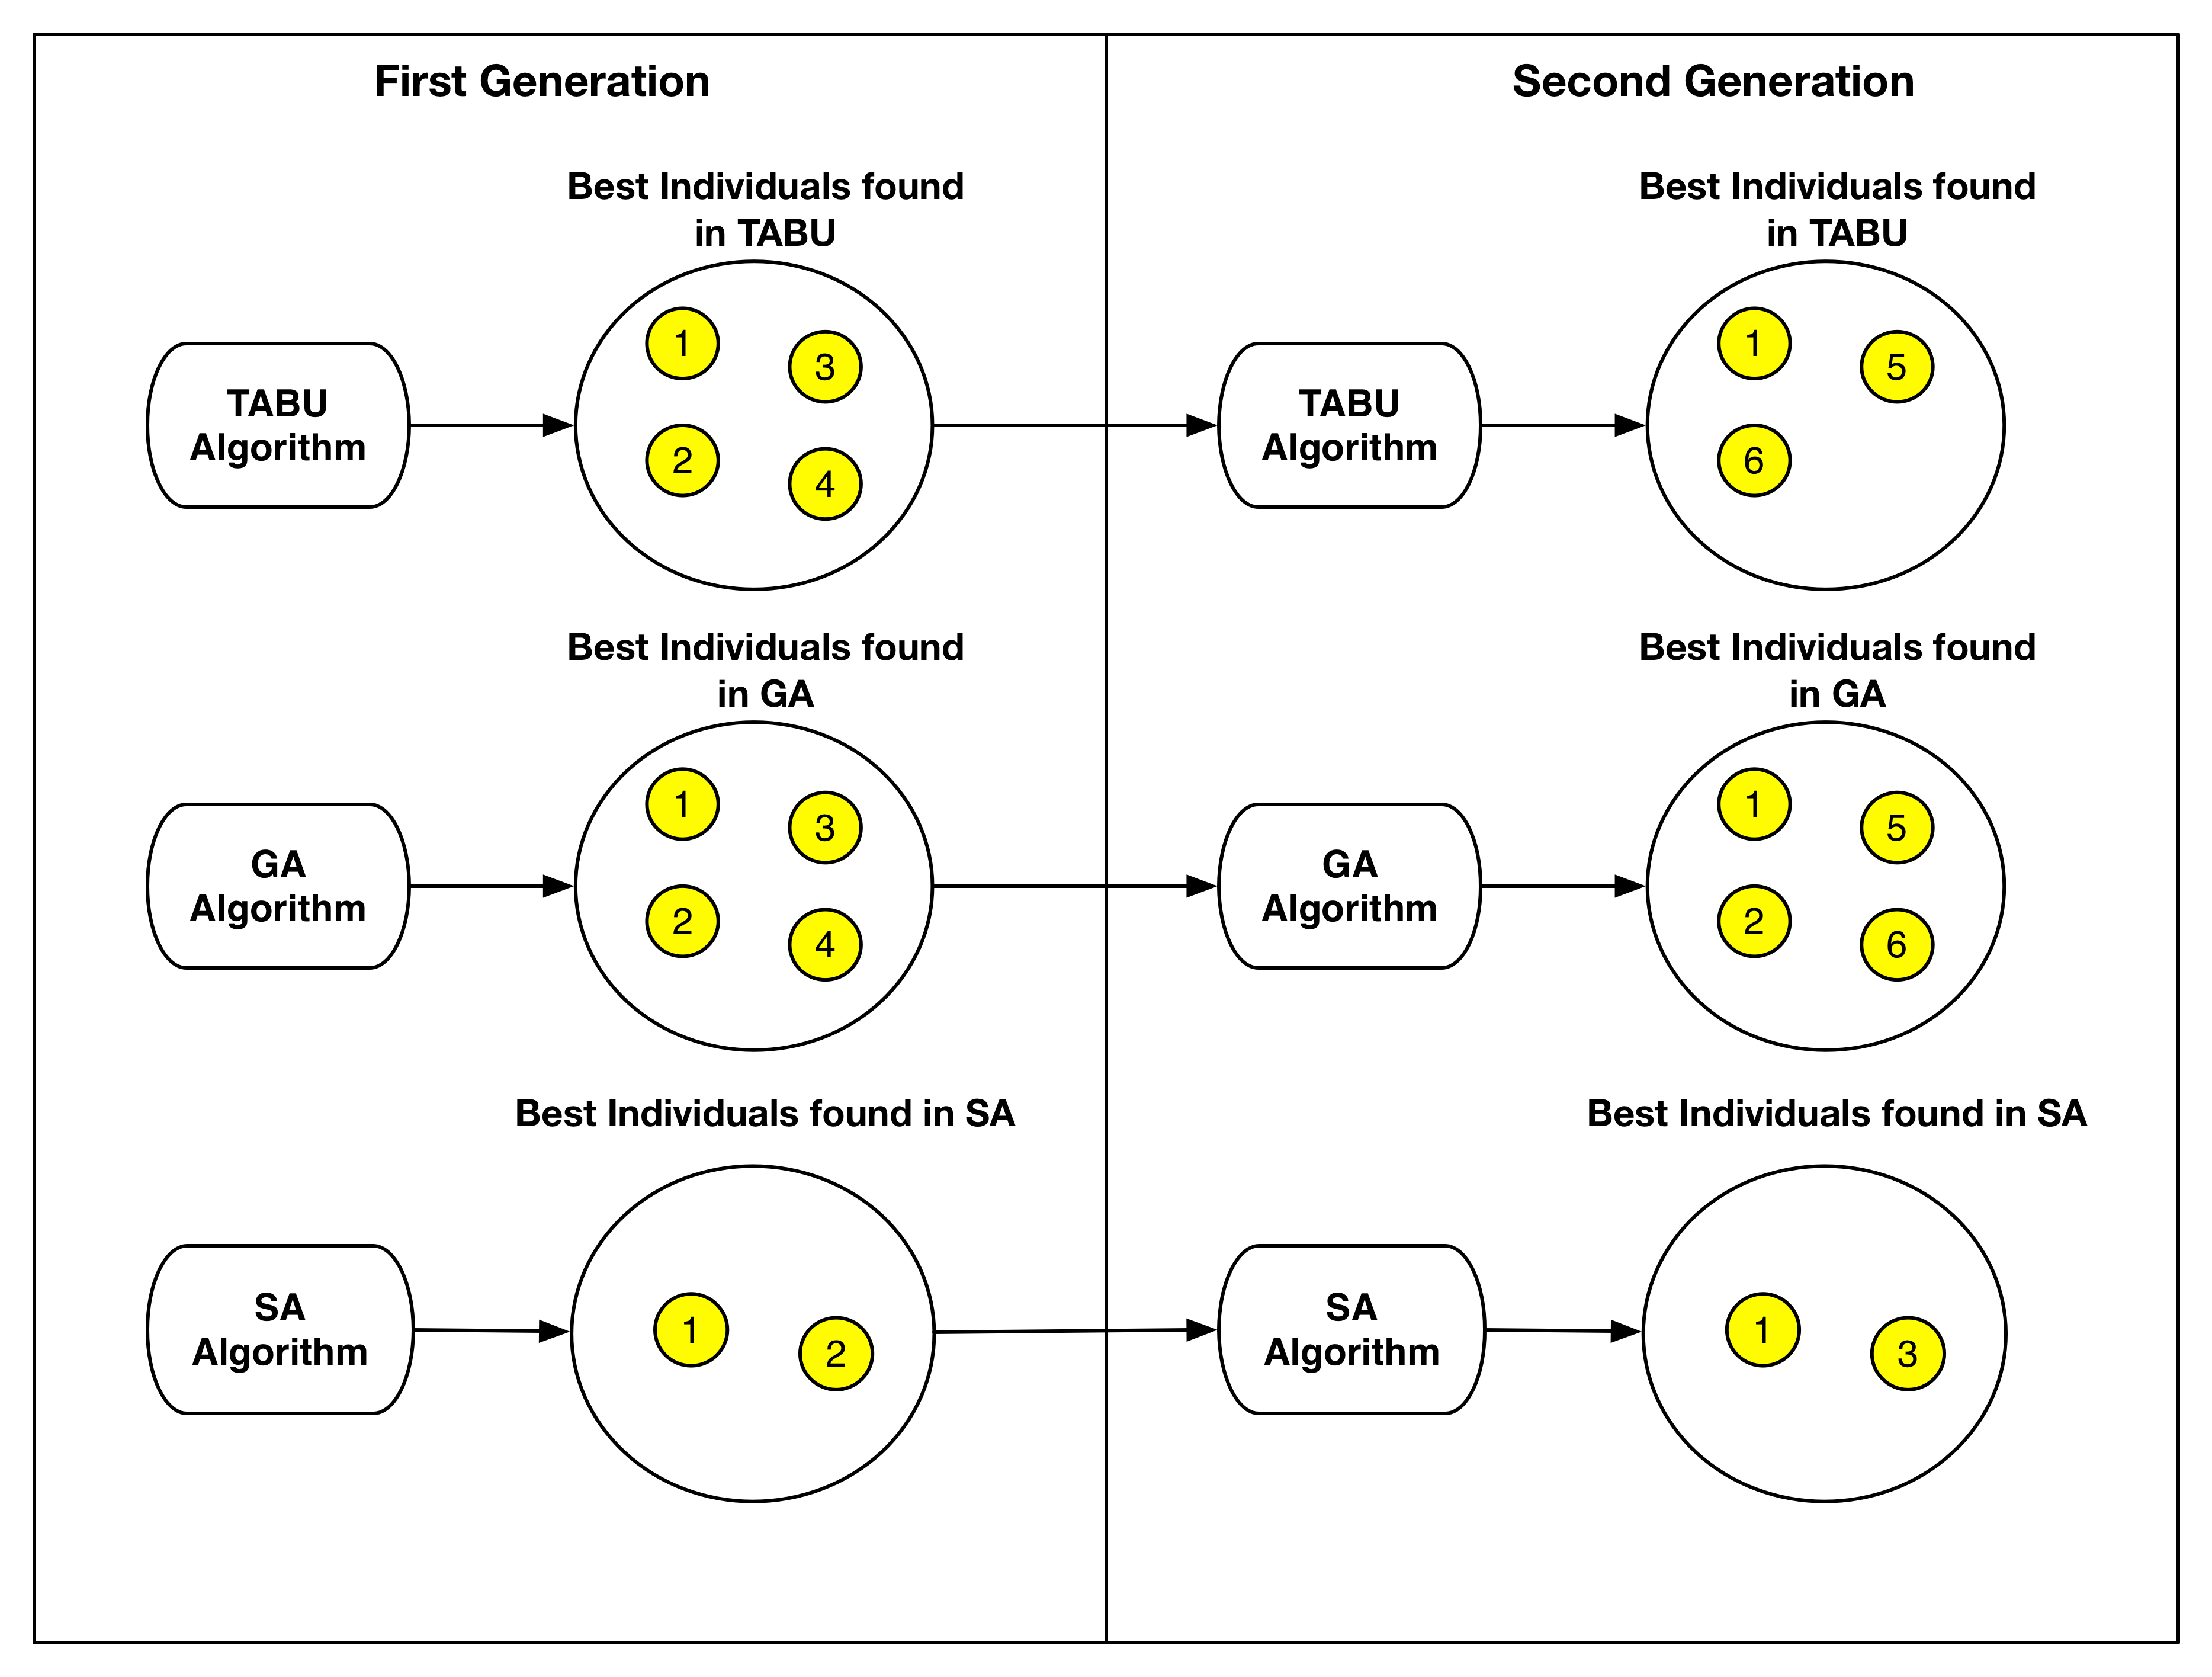
\includegraphics[width=1\textwidth]{./images/independ.png}
\caption{Use of the algorithms independently}
\label{fig:firstaproach}
\end{figure}



The second approach uses the algorithms in a collaborative mode (hybrid metaheuristic). In this approach, the three algorithms share their best individuals found (Fig. \ref{fig:secondapproach}).

The next subsections present details about the used metaheuristic algorithms (Representation, initial population and fitness function).




\begin{figure}
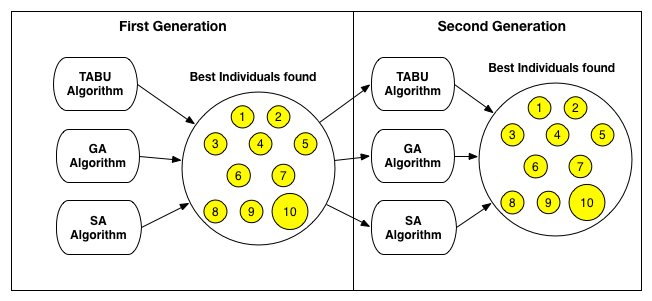
\includegraphics[width=1\textwidth]{./images/collaborative.png}
\caption{Use of the  algorithms collaboratively}
\label{fig:secondapproach}
\end{figure}

\subsection{Representation}

The solution representation is composed by a linear vector with 23 positions. The first position represents the name of an individual. The second position represents the algorithm (genetic algorithm, simulated annealing, or Tabu search) used by the individual. The third position represents the type of test (load, stress, or performance). The next positions represent 10 scenarios and their numbers of users. Each scenario is an atomic operation: the scenario must log into the application, run the task goal, and undo any changes performed, returning the application to its original state.

Fig. \ref{fig:genomarepresentation} presents the solution representation and an example using the crossover operation. In the example, genotype 1 has the Login scenario with 2 users, the Form scenario with 0 users, and the Search scenario with 3 users. Genotype 2 has the Delete scenario with 10 users, the Search scenario with 0 users, and the Include scenario with 5 users. After the crossover operation, we obtain a genotype with the Login scenario with 2 users, the Search scenario with 0 users, and the Include scenario with 5 users.

\begin{figure}[h]
\centering
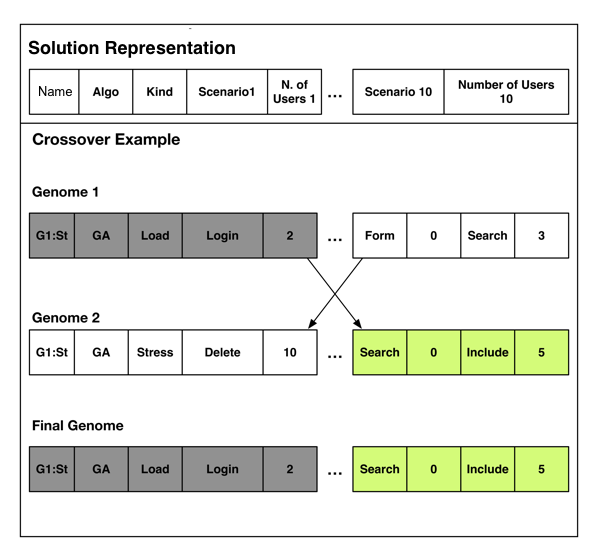
\includegraphics[width=1\textwidth]{./images/genomerepresentation1.png}
\caption{Solution representation and crossover example}
\label{fig:genomarepresentation}
\end{figure}

Fig. \ref{fig:neighbourtaby} shows the strategy used by the proposed solution to obtain the representation of the neighbors for the Tabu search and simulated annealing algorithms. The neighbors are obtained by the modification of a single position (scenario or number of users) in the vector.


\begin{figure}[h]
\centering
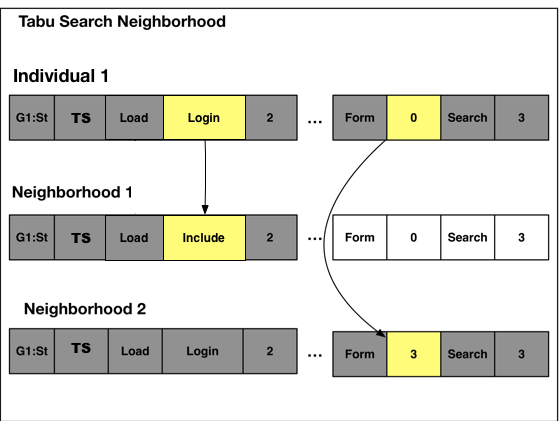
\includegraphics[width=1\textwidth]{./images/TabuNE2.png}
\caption{Tabu search and simulated annealing neighbor strategy}
\label{fig:neighbourtaby}
\end{figure}


\subsection{Initial population}

The strategy used by the plugin to instantiate the initial population is to generate 50\% of the individuals randomly, and 50\% of the initial population is distributed in three ranges of values:

\begin{itemize}
\item Thirty percent of the maximum allowed users in the test;
\item Sixty percent of the maximum allowed users in the test; and
\item Ninety percent of the maximum allowed users in the test.
\end{itemize}

The percentages relates to the distribution of the users in the initial test scenarios of the solution. For example, in a hypothetical test with 100 users, the solution will create initial test scenarios with 30, 60 and 90 users.

\subsection{Objective (fitness) function}

The proposed solution was designed to be used with independent testing teams in various situations where the teams have no direct access to the environment where the application under test was installed. Therefore, the IAdapter plugin uses a measurement approach to the definition of the fitness function. The fitness function applied to the IAdapter solution is governed by the following equation:

\begin{equation}
\begin{aligned}
fit=90percentileweigth* 90percentiletime\\
+80percentileweigth*80percentiletime\\+
70percentileweigth*70percentiletime+\\
maxResponseWeigth*maxResponseTime+\\
numberOfUsersWeigth*numberOfUsers-penalty
\end{aligned}
\end{equation}

The proposed solution's fitness function uses a series of manually adjustable user-defined weights (90percentileweight, 80percentileweight,  70percentileweight, maxResponseWeight, and numberOfUsersWeight). These weights make it possible to customize the search plugin's functionality. A penalty is applied when an application under test takes a longer time to respond than the level of service.

